\documentclass[12pt]{article}
\usepackage[utf8]{inputenc}

\usepackage{enumerate}
\usepackage{listings}
\usepackage{pgfplots}
\usepackage{tikz}
\usepackage{svg}
\usepackage{graphicx}
\usepackage{setspace}
\usepackage{makecell}
\usepackage{caption}
\usepackage{subcaption}
\usepackage{pgf-umlsd}
\usepackage{epstopdf}
\usepackage{bytefield}
\usepackage{amsmath}
\usepackage{csquotes}
\usepackage[nottoc,numbib]{tocbibind}
\usepackage[section]{placeins}
\usepackage{tgtermes}
\usepackage{color}
\usepackage{hyperref}

\usetikzlibrary{shapes.geometric}
\usetikzlibrary{decorations.text}
\usetikzlibrary{positioning}
\usetikzlibrary{fit,shapes}

\hypersetup{
colorlinks,
citecolor=black,
filecolor=black,
linkcolor=black,
urlcolor=black
}

\lstloadlanguages{TeX}

\definecolor{lightred}{rgb}{1,0.7,0.71}

\begin{document}

    \thispagestyle{empty}
{\fontfamily{qtm}\selectfont
\begin{figure}[htbp]
    \centering
    \includegraphics[scale=1.5]{img/agh-logo.pdf}
\end{figure}

\centerline{\small\textbf{AKADEMIA GÓRNICZO-HUTNICZA IM. STANISŁAWA STASZICA W KRAKOWIE}}
\vspace{1em}
\centerline{\small\textbf{WYDZIAŁ INFORMATYKI, ELEKTRONIKI I TELEKOMUNIKACJI}}
\vspace{1em}
\centerline{\small INSTYTUT Informatyki}
\vspace{2em}
\centerline{\Large Praca dyplomowa}
\vspace{2em}
\centerline{\textit{\large Validation of QUIC protocol usefullness in interactive communication}}
\vspace{1em}
\centerline{\textit{\large Ocena przydatności protokołu QUIC w komunikacji interaktywnej}}
\vspace{3em}

\begin{table}[h]
    \begin{tabular}{l l}
        Autor             & Michał Śledź              \\
        Kierunek studiów: & Informatyka               \\
        Opiekun pracy:    & dr inż.\ Łukasz Czekierda \\
    \end{tabular}
\end{table}

\null
\vfill
\centerline{Kraków, 2021}
}
    \clearpage

    \tableofcontents
    \clearpage

    \section{Introduction}
\label{sec:introduction}

An interactive communication is bidirectional data exchange between people or people and machines.
It consists of two or more participants and has to be responsive meaning the result of performed action is delivered almost immediately.
In many cases interactive communication has to be also secure and reliable.
Examples of interactive communication are controlling remote robot in tele-surgery, doing exercises in tele-rehabilitation and
some types of multimedia sessions e.g.\ video conference, collaborative work or chat.
On the other hand to interactive communication does not belong exchanging emails (time between subsequent messages is too big) or
video on demand and streaming (they are not bidirectional).

Years of researches, protocol improvements and network devices optimizations have made interactive communication really fast.
We can talk with another person almost in the real time with a delay of several milliseconds.
Having said that it is perfectly correct to ask a question whether communication can be even faster, more effective and reliable and whether it is still worth to make improvements while we already have well prospering ecosystem.
In 2006 Prof.\ Edward Delp said:
\begin{displayquote}
    Is video coding dead?
    Some feel that, with the higher coding efficiency of the H.264/MPEG-4 Advanced Video Coding (AVC) standard (2x as compared to MPEG-2), perhaps there is not much more to do.
    I must admit that I have heard this \textquote{compression is dead} argument at least four times since I started working in image and video coding in 1976.\cite{4015574}
\end{displayquote}
Despite the fact that we are able to achieve very good performance in video conferencing systems there is still much to do.
Serious gaming, tele-surgery and tele-rehabilitation are all subject to tactile internet in which reliability, security and low latency are fundamental.
In such cases delay of 1 ms is desirable~\cite{the-tactile-internet}.

On the other hand, complexity of current standards makes them hard to implement, monitor and maintain.
One of them is WebRTC which uses over 10 different protocols and leaves implementation of signalling plane to the user.

QUIC is a new transport protocol standardized in RFC 9000 on May in 2021 and provides interesting and promising set of features.
%Its integration with TLS 1.3 significantly reduces connection establishment time while stream multiplexing in a single connection resolves head of line blocking problem of HTTP/2.
%QUIC introduces also special connection identifiers that prevents from additional handshakes in case of network switching and defines own flow control and congestion control mechanisms that are based on TCP ones.
%QUIC packets are encapsulated in UDP datagrams which makes QUIC user level protocol i.e.\ there is no need to modify kernel implementation to provide operating system with support for QUIC\@.
%
QUIC is mostly deployed in conjunction with a new version of HTTP called HTTP/3 and is intended to replace TCP and HTTP/2.
Therefore most publications are focused on web domain comparing QUIC and HTTP/3 with TCP/TLS and HTTP/2.

However, it turns out that a lot of QUIC features mainly stream multiplexing, pluggable congestion control, integration with TLS 1.3
or enhanced connection establishment mechanism can be useful in other domains.
As a result a number of IETF drafts emerged to expand QUIC to new areas.
The most important one is \textit{An Unreliable Datagram Extension to QUIC}.
It allows for combining reliable and unreliable data exchange in the same QUIC connection.

This document tries to answer a question whether QUIC can introduce significant improvement in terms of interactive communication.
To this end, analysis of QUIC encryption, loss detection and flow control mechanisms as well as number of tests and experiments have been performed.

The structure of this document is as follows.
Section~\ref{sec:state-of-the-art} presents state of the art and defines problems that will be addressed in this document.
Section~\ref{sec:quic-overview} introduces basic concepts of QUIC and compares QUIC to other transport protocols.
Section~\ref{sec:quic-in-webrtc} presents how QUIC can simplify WebRTC protocol stack.
It also describes packet encryption process in QUIC, answers the question if header encryption introduces significant overhead to the whole packet encryption and compares QUIC encryption process with RTP one.
Section~\ref{sec:datagrams} is dedicated to DATAGRAM frames in QUIC -- how they work and behave in different scenarios.
Section~\ref{sec:conclusions} concludes this document.

    \clearpage
    %! suppress = EscapeAmpersand


\chapter{QUIC overview}
\label{ch:quic-overview}
QUIC is a connection-oriented, multistream protocol that uses UDP/IP under the hood.
It is integrated with TLS and provides own congestion control and flow control mechanisms.
Data sent over QUIC is delivered in a reliable way.

This section outlines main features of QUIC and compares QUIC to the other transport protocols.


\section{Connection}
\label{sec:connection}
A QUIC connection is shared state between a client and a server.
It consists of connection parameters like initial flow control limit or initial maximal number of streams and
shared secret used for encryption.
Each connection possesses a set of connection identifiers each of which identifies the connection.
The role of connection IDs is to make QUIC connection resilient for changes in addressing at lower protocol layers (UDP, IP).
In such scenarios, as long as there is an alternative network path QUIC can migrate to it without restarting the connection.
As an example one could open UDP socket, establish QUIC connection, start sending packets using open socket and after some time
switch UDP socket to another one (e.g.\ because of moving train) without re-establishing QUIC connection or creating a new one.

Using a connection ID is optional and an endpoint can decide to use zero-length connection ID when a connection ID is not needed to route packets to the correct endpoint.
However, choosing zero-length connection ID makes it impossible to use some QUIC features like mentioned above
connection migration.


\section{Data structures}
\label{sec:quic-data-structures}
The most outer entity in QUIC is a packet.
QUIC defines different types of packets each of which consists of a header followed by a type-specific payload.

Header can take long or short form.
Packets with long headers are used at the beginning of the communication, before establishing 1-RTT keys.
After negotiating cryptographic context QUIC switches to the packet type with short header form for minimizing data sent
through the network.
Short Header consists of miscellaneous flags which take one byte, destination connection ID and packet number.
Total size of Short Header depends on using zero-length connection ID and is from 2 to 25 bytes allowing for saving
bandwidth in scenarios when some QUIC features like connection migration are not needed.
Short header form is illustrated in figure~\ref{fig:short-header-format}.

\begin{figure}[h]
    \centering
    \begin{bytefield}[bitwidth=4em]{8}
        \bitheader{0-7} \\
        \bitbox{1}{\tiny header form} & \bitbox{1}{\tiny fixed bit} & \bitbox{1}{\tiny spin bit} & \bitbox{2}{\tiny reserved bits} & \bitbox{1}{\tiny key phase} & \bitbox{2}{\tiny packet number length} \\
        \wordbox{1}{\tiny destination connection ID (0 - 160)} \\
        \wordbox{1}{\tiny packet number (8 - 32)}
    \end{bytefield}
    \caption{QUIC Short Header format}
    \label{fig:short-header-format}
\end{figure}

Long Header additionally includes version, destination connection ID length, source connection ID
length and source connection ID fields.
It does not include packet number field and its flags differ a little comparing to the Short Header but they also take 1 byte.
Total length of Long Header also depends on using zero-length connection ID and is from 7 to 47 bytes.
Long header form is illustrated in figure~\ref{fig:long-header-format}.

\begin{figure}[h]
    \centering
    \begin{bytefield}[bitwidth=4em]{8}
        \bitheader{0-7} \\
        \bitbox{1}{\tiny header form} & \bitbox{1}{\tiny fixed bit} & \bitbox{2}{\tiny long packet type} & \bitbox{4}{\tiny Type-Specific Bits} \\
        \wordbox{4}{\tiny Version (32)} \\
        \wordbox{1}{\tiny Destination Connection ID Length} \\
        \wordbox{1}{\tiny destination connection ID (0 - 160)} \\
        \wordbox{1}{\tiny Source Connection ID Length} \\
        \wordbox{1}{\tiny Source Connection ID (0 - 160)}
    \end{bytefield}
    \caption{QUIC Long Header format}
    \label{fig:long-header-format}
\end{figure}

QUIC defines following types of packets that use long header form: Version Negotiation, Initial, 0-RTT, Handshake, Retry and one packet type that uses short header form called 1-RTT\@.

Payload form depends on a packet type.
It includes type-specific fields which are in most cases followed by QUIC frames.
Payload can include many frames and many frame types.
Some of the QUIC frames are: PING, ACK, CRYPTO or STREAM\@.
Different frame types can appear only in specific packet types.
For example STREAM frame can only be included in 0-RTT or 1-RTT packets while CRYPTO frame can appear in Initial, Handshake or 1-RTT packets.
Version Negotiation and Retry packets does not include any QUIC frames at all.


\section{Encapsulation}
\label{sec:udp-based}
QUIC packets are directly encapsulated into UDP datagrams.
One UDP datagram can coalesce multiple QUIC packets provided that each of them possesses the same connection ID and contains length field.
If a packet does not contain length field it has to be placed at the end of UDP datagram which implies there can be only one such packet.
Packets that contain length field are Initial, 0-RTT and Handshake while packets without length field are Retry, Version Negotiation
and 1-RTT\@.
It is also important that there is no situation where Retry or Version Negotiation packet is coalesced with another packet.
One of the advantages of coalescing QUIC packet is reduction of number of UDP datagrams needed to establish QUIC connection.
Example encapsulation is shown in figure~\ref{fig:quic-encapsulation}.

\begin{figure}[h]
    \centering
    \begin{bytefield}[bitwidth=4em]{8}
        \begin{leftwordgroup}{\small UDP \\ \small header}
            \bitbox{4}{\small Source Port} & \bitbox{4}{\small Destination Port} \\
            \bitbox{4}{\small Length } & \bitbox{4}{\small Checksum}
        \end{leftwordgroup} \\
        \begin{leftwordgroup}{\small UDP \\ \small payload}
            \wordbox{1}{\small QUIC Long Header packet} \\
            \wordbox{1}{\small QUIC Long Header packet} \\
            \wordbox{1}{\small QUIC Short Header packet}
        \end{leftwordgroup}
    \end{bytefield}
    \caption{QUIC encapsulation into UDP datagram}
    \label{fig:quic-encapsulation}
\end{figure}

Encapsulating QUIC packets into UDP datagrams makes QUIC user-level protocol which means it can be implement as a usual
library without modifying operating system kernel.
Moreover, existing middleboxes see QUIC packets as usual UDP datagrams and do not require providing support for a new protocol.
On the other hand, a lot of government institutions as well as companies block incoming or outgoing UDP traffic and allow
only for communication via TCP or TLS on port 443.


\section{Security}
\label{sec:security}
QUIC is integrated with TLS 1.3 providing confidentiality, integrity and authenticity of its packets.
Confidentiality means that no one is able to decrypt data being sent to the other endpoint, integrity means that no one
is able to modify this data and authenticity means that each endpoint can verify identity of
its peer to be sure that it is communicating with proper entity.
Integration with TLS 1.3 is described in details in RFC 9001~\cite{rfc9001}.
Both transport and cryptographic parameters are negotiated in a single connection handshake which results in
reduction of connection establishment time (see~\ref{sec:connection-establishment}).
Unlike in TLS over TCP, QUIC does not carry TLS records.
Instead, TLS handshake and alert messages are encapsulated directly into QUIC packets.
This includes sending casual data over QUIC -- it does not use TLS Application Data record but QUIC frames.
Figure~\ref{fig:quic-tls-interactions} shows interactions between QUIC and TLS\@.
Both protocols cooperate: QUIC receives cryptographic keys which are then used to protect packets by QUIC itself whereas
TLS uses QUIC reliability and record layer.

\begin{figure}
    \centering
    \tikzstyle{rect}=[rectangle,minimum width=3cm,minimum height=3cm,draw=black]
    \begin{tikzpicture}

        \node[rect] (quic) {QUIC};
        \node[rect,below=2cm of quic,align=center] (quic-packet-protection) {QUIC \\ Packet \\ Protection};
        \node[rect,right=5cm of quic] (tls) {TLS};

        \draw [<->, postaction={decorate,decoration={raise=0.5ex,text along path,text align=center,text={Handshake Parameters}}}] (1.5, 1.25) -- (6.5, 1.25);
        \draw [<->, postaction={decorate,decoration={raise=0.5ex,text along path,text align=center,text={Validate 0-RTT Keys}}}] (1.5, 0.75) -- (6.5, 0.75);
        \draw [<-, postaction={decorate,decoration={raise=0.5ex,text along path,text align=center,text={0-RTT Keys}}}] (1.5, 0.25) -- (6.5, 0.25);
        \draw [<-, postaction={decorate,decoration={raise=0.5ex,text along path,text align=center,text={Handshake Keys}}}] (1.5, -0.25) -- (6.5, -0.25);
        \draw [<-, postaction={decorate,decoration={raise=0.5ex,text along path,text align=center,text={1-RTT Keys}}}] (1.5, -0.75) -- (6.5, -0.75);
        \draw [<-, postaction={decorate,decoration={raise=0.5ex,text along path,text align=center,text={Handshake Done}}}] (1.5, -1.25) -- (6.5, -1.25);

        \draw [->] (-1, -1.5) to node[align=center,left] {Protect} (-1, -3.5);
        \draw [<-] (1, -1.5) to node[align=center,right] {Protected \\ Packet} (1, -3.5);
    \end{tikzpicture}
    \caption{QUIC and TLS interactions (Figure 4 from RFC 9001, Section 3)}
    \label{fig:quic-tls-interactions}
\end{figure}

Encryption in QUIC is mandatory which means there is no possibility to send unencrypted data.
Encryption process includes payload and partially header of QUIC packet (see section~\ref{sec:packet-encryption-overhead}).
One of the questions this thesis aims to answer is whether QUIC encryption scheme introduces a significant overhead to the interactive communication.


\section{Connection establishment}
\label{sec:connection-establishment}
Combining transport and cryptographic handshake results in significant reduction of connection establishment time.
Figure~\ref{fig:low-latency-conn-est} compares time needed for sending HTTP request using TCP/TLS and QUIC\@.

\begin{figure}[h]
    \centering
    \begin{subfigure}{.5\textwidth}
        \begin{sequencediagram}
            \newinst{client}{Client}
            \newinst[3]{server}{Server}
            \mess{client}{TCP SYN}{server}
            \mess{server}{TCP SYN + ACK}{client}
            \mess{client}{TCP ACK}{server}
            \postlevel
            \mess{client}{TLS ClientHello}{server}
            \mess{server}{TLS ServerHello}{client}
            \mess{client}{TLS Finished}{server}
            \postlevel
            \mess{client}{HTTP REQ}{server}
            \mess{server}{HTTP RES}{client}
        \end{sequencediagram}
        \caption{HTTP request in TCP}
        \label{subfig:http-req-tcp}
    \end{subfigure}%
    \begin{subfigure}{.5\textwidth}
        \begin{sequencediagram}
            \newinst{client}{Client}
            \newinst[3]{server}{Server}
            \mess{client}{QUIC}{server}
            \mess{server}{QUIC}{client}
            \mess{client}{QUIC}{server}
            \postlevel
            \mess{client}{HTTP REQ}{server}
            \mess{server}{HTTP RES}{client}
        \end{sequencediagram}
        \caption{HTTP request in QUIC}
        \label{subfig:http-req-quic}
    \end{subfigure}
    \caption{HTTP request comparison between TCP/TLS and QUIC}
    \label{fig:low-latency-conn-est}
\end{figure}

Round Trip Time (RTT) is a time needed for transporting a message from one side to the other and back again.
Standard HTTP request using TCP/TLS stack requires 3-RTT -- one for TCP handshake, one for TLS handshake and one for HTTP request.
Even though TCP handshake sends 3 messages it is still counted as 1-RTT as there is no need to wait for a response to the last message.
Instead, we can immediately send next data which is in this case data for TLS handshake.

QUIC takes another approach.
It combines transport and cryptographic handshakes reducing time needed for establishing a connection.
In such a case sending an HTTP request occurs after 1-RTT\@.
The whole communication lasts 2-RTT\@.

In some scenarios, when there was communication with the server previously and client cached information from it QUIC can
reduce time needed for sending an HTTP request and receiving a response even more.
To this end 0-RTT packets are used.
They allow to send application data in 0-RTT (together with handshake parameters) reducing the whole communication to 1-RTT\@.
0-RTT HTTP request is presented in figure~\ref{fig:http-req-quic-0rtt}
\begin{figure}[h]
    \centering
    \begin{sequencediagram}
        \newinst{client}{Client}
        \newinst[3]{server}{Server}
        \mess{client}{QUIC}{server}
        \mess{client}{HTTP REQ}{server}
        \postlevel
        \mess{server}{QUIC}{client}
        \mess{server}{HTTP RES}{client}
        \postlevel
        \mess{client}{QUIC}{server}
    \end{sequencediagram}
    \caption{HTTP request in QUIC with 0-RTT packets}
    \label{fig:http-req-quic-0rtt}
\end{figure}

\FloatBarrier


\section{Streams}
\label{sec:streams}
Stream is an ordered sequence of bytes.
Each stream can be unidirectional or bidirectional and can be opened by a client or by a server.
Different types of streams can have different flow control limits (see section~\ref{sec:flow-control-and-congestion-control}).
QUIC streams are managed by special types of frames mainly by STREAM frames.
In particular, one STREAM frame can open stream, carry some data and close this stream.
Other frame types related to streams are e.g.\ MAX\_STREAM\_DATA or STREAM\_DATA\_BLOCKED which are used for managing flow control limits.

Type of stream is denoted by proper stream ID which is a 62 bit integer.
The last significant bit identifies the initiator of the stream -- 0 means client initiated stream whereas 1 means server
initiated stream.
The second last significant bit distinguishes between bidirectional streams which have this bit set to 0 and unidirectional streams
which have this bit set to 1.
As an example, stream ID 2 means it is client initiated, unidirectional stream while stream ID 3 and 7 are server initiated,
also unidirectional streams.

An QUIC implementation should also provide means to define stream priority however, information about this priority has to come
from application layer -- QUIC does not define means to exchange stream priority information.
Data that belongs to streams with higher priority will be put on the wire before streams with lower priority.
Prioritization scheme is shown in details in figure~\ref{fig:stream-prioritization}.
Client connects to server and opens one unidirectional stream that can be used to request data of specified type.
If service that client is communicating with is for example website with video-on-demand then client can ask server
application to send it media data at first and when it fills its video buffer it can switch to downloading HTML\@.
This way, using stream multiplexing and prioritization mechanisms client can reduce initial buffering time.

\begin{figure}[h]
    \centering
    \tikzstyle{rect}=[rectangle,minimum width=2cm,minimum height=4cm,draw=black]
    \begin{tikzpicture}

        \node[rect,align=center] (client-quic) {Client \\ QUIC};
        \node[rect,left=1.5cm of client-quic,align=center] (client) {Client \\ Application};
        \node[rect,right=3cm of client-quic,align=center] (server) {Server \\ QUIC};
        \node[rect,right=1.5cm of server,align=center] (server-quic) {Server \\ Application};

        \draw [->,color=olive] (-2.5, 1.5) to node[align=center,above] {give me\\media} (-1, 1.5);
        \draw [<-,color=blue] (-2.5, 0) to node[align=center,above] {media} (-1, 0);
        \draw [<-,color=red] (-2.5, -1.5) to node[align=center,above] {html} (-1, -1.5);

        \draw [->,color=olive] (1, 1.5) to node[align=center,above] {stream 2} (4, 1.5);
        \draw [<-,color=blue] (1, 0) to node[align=center,above] {stream 3:media\\prio:high} (4, 0);
        \draw [<-,color=red] (1, -1.5) to node[align=center,above] {stream 7:html\\prio:low} (4, -1.5);

        \draw [->,color=olive] (6, 1.5) to node[align=center,above] {give me\\media} (7.5, 1.5);
        \draw [<-,color=blue] (6, 0) to node[align=center,above] {set high\\prio} (7.5, 0);
        \draw [<-,color=red] (6, -1.5) to node[align=center,above] {set low\\prio} (7.5, -1.5);
    \end{tikzpicture}
    \caption{QUIC and TLS interactions (Figure 4 from RFC 9001, Section 3)}
    \label{fig:stream-prioritization}
\end{figure}

Another feature of QUIC streams is that they carry data independently which means that losing packet in one stream does not affect flow in other streams.
Figure~\ref{fig:stream-multiplexing} shows this scenario.
One of the packets in stream 1 (marked as gray) was lost and needs to be retransmitted blocking subsequent packets (marked as black) on the receiver side.
They cannot be conveyed to the application layer until retransmission and reordering of the lost packet.
This is the source of so called head of line blocking problem which appears when we are trying to multiplex many HTTP requests in a single TCP connection.
Losing one packet stops the entire flow.
However, thanks to the stream multiplexing QUIC resolves this problem and streams 2 and 3 are not affected by the packet loss in stream 1.

\begin{figure}[h]
    \centering
    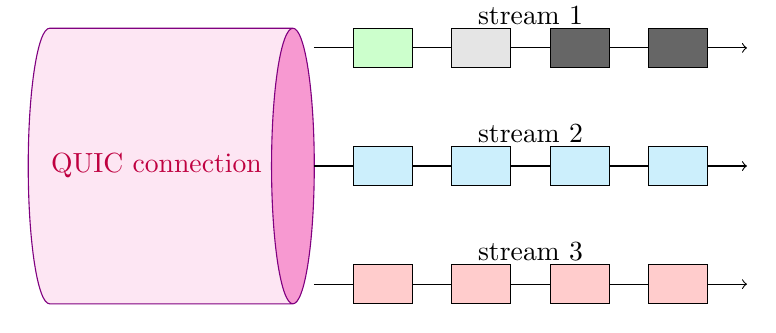
\begin{tikzpicture}

        \node[cylinder,
        draw = violet,
        text = purple,
        style={transform shape},
        cylinder uses custom fill,
        cylinder body fill = magenta!10,
        cylinder end fill = magenta!40,
        minimum size = 3.5cm] (c) at (0,0) {QUIC connection};

        \draw [->, postaction={decorate,decoration={raise=2ex, text along path,text align=center,text={stream 1}}}] (2, 1.5) -- (7.5, 1.5);
        \filldraw [fill=green!20, draw=black] (2.5, 1.25) rectangle (3.25, 1.75);
        \filldraw [fill=gray!20, draw=black] (3.75, 1.25) rectangle (4.5, 1.75);
        \filldraw [fill=black!60, draw=black] (5, 1.25) rectangle (5.75, 1.75);
        \filldraw [fill=black!60, draw=black] (6.25, 1.25) rectangle (7, 1.75);

        \draw [->, postaction={decorate,decoration={raise=2ex, text along path,text align=center,text={stream 2}}}] (2, 0) -- (7.5, 0);
        \filldraw [fill=cyan!20, draw=black] (2.5, -0.25) rectangle (3.25, 0.25);
        \filldraw [fill=cyan!20, draw=black] (3.75, -0.25) rectangle (4.5, 0.25);
        \filldraw [fill=cyan!20, draw=black] (5, -0.25) rectangle (5.75, 0.25);
        \filldraw [fill=cyan!20, draw=black] (6.25, -0.25) rectangle (7, 0.25);

        \draw [->, postaction={decorate,decoration={raise=2ex, text along path,text align=center,text={stream 3}}}] (2, -1.5) -- (7.5, -1.5);
        \filldraw [fill=red!20, draw=black] (2.5, -1.75) rectangle (3.25, -1.25);
        \filldraw [fill=red!20, draw=black] (3.75, -1.75) rectangle (4.5, -1.25);
        \filldraw [fill=red!20, draw=black] (5, -1.75) rectangle (5.75, -1.25);
        \filldraw [fill=red!20, draw=black] (6.25, -1.75) rectangle (7, -1.25);


    \end{tikzpicture}
    \caption{Stream multiplexing in a single QUIC connection}
    \label{fig:stream-multiplexing}
\end{figure}


\section{Flow control}
\label{sec:flow-control-and-congestion-control}
Flow control is a mechanism which allows receiver to announce how much data it is able to process/buffer and sender must
not exceed this limit until it is updated.
In QUIC, flow control limits can be set on two levels.
The first one is stream level -- it is set per stream type e.g.\ for all unidirectional streams opened by the peer or for all bidirectional streams opened locally.
There is no possibility to set flow control limit for a stream with a particular id.
The second one is connection level and it limits overall data amount that can be sent within the whole connection across all streams.
QUIC allows also for limiting number of streams that can be opened by the peer.
These limits are also set per stream type -- unidirectional or bidirectional and initiated by a peer or locally.

It might look like smaller granulation of flow control configuration (setting flow control limit per stream instead of
stream type) could provide more flexibility and could fit better in different use cases but similar mechanism can
be achieved using stream prioritization in the way described above (see section~\ref{sec:streams}).


\section{Congestion control}
\label{sec:congestion-control}
Congestion control also limits amount of data that can be transmitted by a sender but instead of protecting receiver it aims to prevent
from overwhelming network middleboxes like routers and if such overwhelm occurs it helps to recover from it.
RFC 9001~\cite{rfc9001} describes in details sender-side QUIC congestion controller similar to TCP NewReno.
It is triggered when one of QUIC packets is lost or when sender receives IP packet with ECN-CE flag set.
ECN stands for Explicit Congestion Notification while CE stand for Congestion Experienced and it is a codepoint (0x11) set as
value of two least significant bits of the ToS (Type of Service) field in IP header.
Whenever some middlebox is going to be overwhelmed it sets this flag in packets that it routes from a sender to a receiver.
Receiver then informs sender that the network is overwhelmed also by sending IP packets with ECN-CE flag set.

Besides NewReno QUIC can use any other congestion control algorithm that meets requirements defined in section 3.1 of RFC 8085~\cite{rfc8085}.
This makes QUIC congestion control mechanism pluggable and allows for adapting congestion control algorithm to specific use case.


\section{Reliability}
\label{sec:reliability}
QUIC is a reliable protocol which means it guarantees delivery of each packet sent by the endpoint.
Packets are delivered to the application layer in the order they were sent.
However, there are different IETF drafts that expand QUIC with new features.
One of them called \textit{An Unreliable Datagram Extension to QUIC}\cite{bider-ssh-quic-09} allows for sending unreliable messages over QUIC\@.
This can take place in simultaneously to the reliable communication.
Unreliable messages are not subject to flow control mechanisms however, they are congestion controlled.
Each unreliable message is also acknowledged so that application layer can be provided with the packet loss information.
Section~\ref{sec:partial-reliability} describes Datagram extension in details.


\section{Other transport protocols}
\label{sec:other-transport-protocols}
This section compares QUIC with three main transport protocols -- TCP, UDP and SCTP\@.

\subsection{TCP}
\label{subsec:tcp}
Transmission Control Protocol -- connection-oriented, stream oriented and reliable transport protocol.
It guarantees the order of messages and provides flow control and congestion control mechanisms.
TCP is not a multiplexed protocol.
In one TCP connection we have one logical communication channel.
This is the reason of head of line blocking problem that appears when many HTTP/2 requests are multiplexed in one TCP connection.
Because of its reliability, TCP is not a good choice for many types of interactive communication.

\subsection{UDP}
\label{subsec:udp}
User Datagram Protocol -- connection less, unreliable transport protocol.
It does not ensure that messages are delivered in the same order they were sent.
Datagrams, in this protocol, are not acknowledged nor congestion controlled.
It does not also introduce any flow control mechanisms.
Thanks to its simplicity and low bandwidth affection it is the base for RTP protocol which is widely used for transmitting multimedia.
Unlike TCP, UDP also allows for multicast transmission.
However, multicast is rarely used, mostly in local networks.

\subsection{SCTP}
\label{subsec:sctp}
Stream Control Transmission Protocol -- reliable, message oriented transport protocol.
Messages in SCTP can be delivered in order or out of order which is indicated by \textit{U} flag in DATA chunk.
DATA chunk can be thought as similar entity to QUIC frame and it can contain either control information or user data.
Chunks with \textit{U} flag set to 1 are immediately conveyed to the upper layer.
In particular setting \textit{U} flag to 1 for each DATA chunk makes whole communication unordered.
Unlike TCP and similarly to QUIC, SCTP is multistream protocol -- it allows for opening multiple logical streams in one physical connection.
Another feature of SCTP is multi-homing in which an endpoint uses two different addresses introducing some kind of fault tolerance --
one address is designated as a primary and the other one can be used in case of failure of the first one.
SCTP operates on connection less packet network such as IP therefore it needs dedicated support in middleboxes so that they can
recognize its packets correctly.
Lack of this support led to the fact that SCTP was not implemented on a mass scale and its main domain is telecommunication.
This is something that QUIC does not repeat as QUIC packets are seen by routers as usual UDP datagrams.

\subsection{Summary}
\label{subsec:summary}
Table~\ref{tab:protocols_comparision} presents a short summary of transport protocols comparison.
\begin{table}[h]
    \centering
    \resizebox{\columnwidth}{!}{%
    \begin{tabular}{|c | c | c | c | c |}
        \hline
        & TCP           & UDP              & SCTP                                   & QUIC                           \\
        \hline
        reliability        & reliable      & unreliable       & unreliable/partially reliable/reliable & unreliable/reliable            \\
        \hline
        transmission       & byte oriented & message oriented & message oriented                       & message oriented/byte oriented \\
        \hline
        flow control       & yes           & no               & yes                                    & only for streams               \\
        \hline
        congestion control & yes           & no               & yes                                    & yes                            \\
        \hline
        packets order      & ordered       & unordered        & unordered/partially ordered/ordered    & unordered/ordered              \\
        \hline
        multistream        & no            & no               & yes                                    & yes                            \\
        \hline
    \end{tabular}%
    }
    \caption{\label{tab:protocols_comparision}Transport protocols comparison.}
\end{table}

    \clearpage
    \section{State of the art}
\label{sec:state-of-the-art}

The number of QUIC publications at the moment of writing this thesis is limited.
The main reason of such situation is that QUIC was standardize just a few months ago.
In this section I present an overview of publications that are important in terms of current main QUIC usage which is
HTTP/3, are somehow related to transporting media over QUIC or are dedicated to aspects that are also important
in interactive communication.

\textit{The QUIC Fix for Optimal Video Streaming} article~\cite{the-quic-fix-for-optimal-video-streaming} introduces unreliable data transmission over QUIC and presents how combination of reliable and unreliable transmission fares in video streaming and outperforms TCP and reliable mode of QUIC\@.
Authors of this document tag H.264 video frames depending on their importance.
\textit{I-Frames} which are independent frames meaning they can be displayed without any additional frames are marked to be sent reliably.
\textit{P-Frames} which are much smaller in size and code only the difference between \textit{I-Frame} and the next frame are marked to be sent unreliably.
The same approach is applied to \textit{B-Frames} that depends on both \textit{I-Frames} and \textit{P-frames}.
Authors state that the loss of \textit{P-Frames} or \textit{B-Frames} has minimal or no impact on the user's quality of experience (QoE).
They use i.a. \textit{buffering ratio (bufRatio)} and \textit{rate of buffering (rateBuf)} metrics to measure the difference in performance of streaming video over codec-agnostic DASH protocol used with TCP, traditional QUIC and QUIC with addition of unreliable transmission.
\textit{BufRatio} is the amount of time spent on re-buffering video comparing to the total video duration, represented as a percentage.
\textit{RateBuf} is the frequency of the buffering events~\cite{impact-of-video-quality-on-user-engagement}.
As a result, \textit{bufRatio}, with packet loss set to 0.64\%, for TCP is 105\%, for QUIC is 30\% and for QUIC with addition of unreliable data transmission is less than 1\%.
\textit{RateBuf}, with the same packet loss, is equal to 50\% for TCP, 19\% for QUIC and nearly 0\% for QUIC with addition of unreliable data transmission.

\textit{QUIC: Better for what and for whom?} article~\cite{quic-better-for-what-and-for-whom} compares the page load time (PLT) for HTTP/2 requests over QUIC and TCP/TLS in different network conditions and architectures as well as for different website complexities.
Authors prepared both local and remote testbeds.
In the remote one client's machine is connected to the Internet over ADSL (to router over Ethernet or Wi-Fi) or 4G\@.
Different network conditions mean different packet loss rate and delay.
In case of complexity of site there is Youtube service in which different resources might be distributed over many servers and Doctor (website of the ANR project) website where ale files are located on the same server.
Authors concludes that QUIC outperforms HTTP/2 over TCP/TLS in unstable networks but in case of stable and reliable networks the benefits of QUIC are not so obvious.

\textit{Game of protocols: Is QUIC ready for prime time streaming?} article~\cite{game-of-protocols} compares QUIC and TCP in HAS (HTTP adaptive streaming) applications.
To this end, authors performed experiments in four scenarios.
Frame-seek scenario is about seeking to the specified frame in the video.
Connection-switch scenario is about changing the connection from e.g.\ Wi-Fi to 3G\@.
Multiplexing scenario is about comparing different stream multiplexing techniques i.e.\ HTTP/1.1 over varying number of TCP connections, HTTP/2 with parallel requests over a single TCP connection and QUIC over a single UDP connection.
Fairness scenario is about checking fairness of congestion control mechanisms while there are multiple competing clients.
Authors also used three different adaptive algorithms: BASIC, SARA and BBA-2.
In the frame-seek scenario QUIC behaved better for all adaptive algorithms and types of networks reducing numerically \textit{rebufferRate} metric (which is a similar metric to \textit{bufRatio}) by 1--3\%.
In the WiFi-LTE and WiFi-3G connection-switch scenario, QUIC also behaved better for all adaptive algorithms reducing numerically \textit{rebufferRate} by 1\% for SARA and BBA-2 and by 7\% for BASIC\@.
Evaluation of different multiplexing techniques showed that in the typical network conditions all three methods resulted in the similar average playback bitrate.
In the large delay and typical loss network, QUIC performed best.
For typical delay and large loss as well as for large delay and large loss, HTTP/1.1 with varying number of TCP connections was better than QUIC\@.
HTTP/2 over single TCP connection didn't manage to beat any of the other multiplexing techniques in any of the network conditions.
Fairness examination of congestion control mechanisms in TCP and QUIC showed that for typical packet loss and delay both protocols guarantee fair resource access for competing clients which results in the similar average playback bitrate.
In the large loss scenario single QUIC client was able to achieve higher bitrate (about 37\%) than single TCP client.
For competing clients, QUIC still was able to achieve better bitrate than TCP (about 40\%).
In the large delay scenario, the results were similar to the large loss scenario.
The last one scenario with large loss and large delay showed that TCP client was able to achieve higher bitrate (about 16\%) both when competing and not competing with QUIC client.

\textit{And QUIC meets IoT: performance assessment of MQTT over QUIC} article~\cite{and-quic-meets-iot} maps MQTT to QUIC
and compares its performance with state-of-the-art MQTT over TCP\@.
Authors performed two tests.
In the first one, they send 1000 MQTT messages to the broker which then are sent to the subscriber.
In the second one, they establish MQTT connection and send only one message and close the connection.
The purpose of the second scenario was to see improvements introduced by QUIC in terms of faster connection establishment.
Both tests were performed in three different, emulated network environments: Wi-Fi, 4G/LTE and Satellite.
Authors states that MQTT over QUIC outperforms MQTT over TCP however, they expected a bigger advantage
of QUIC in the second scenario due to QUIC 0-RTT packets.

\textit{Emerging Interactive Applications over QUIC} article~\cite{9045245} compares QUIC performance with TCP and UDP
using three multimedia services.
The first service which is cloud gaming represents an interactive communication.
The second and third ones which are 4K video streaming and client-server online gaming represent classic multimedia
applications.
Each client in each service was connected to the Access Point which had access to the Internet.
The bottle neck was the connection between AP and router to which three servers (one for each service) were connected.
The first experiment tests QUIC fairness and shows that average achieved bandwidth by Cloud Gaming and 4K streaming
is more balanced when using QUIC\@.
The second experiment tests QUIC end-to-end latency and shows a significant delay reduction for all three services when using QUIC\@.
In the last scenario, authors compare Round Trip Time when streaming 4K video using QUIC and TCP\@.
Experiment shows that RTT for QUIC is lower than for TCP\@.
To sum up in all scenarios QUIC outperforms traditional transport protocols both for interactive and classic multimedia
applications.

\textit{Media QoE Enhancement With QUIC} article~\cite{7562075} uses QUIC stream prioritization to improve Quality of Experience (QoE).
Authors focus on MPEG-DASH based application.
They prioritize streams that carry multimedia data depending on the client's player buffer.
If its level is below 20 sec then client requests subsequent media chunks with high priority.
For buffer level between 20 and 80 sec medium priority is requested and for buffer level above 80 sec high priority.
The experiment shows that stream prioritization gain in Initial Buffering Time can be from 6\% to 49\% depending on
bandwidth limit and video resolution.
%
%\textit{Impact of ACK Scaling Policies on QUIC Performance} article~\cite{9524947}
%
%
%
%\textit{An attempt at introducing Multipath in QUIC} article~\cite{8806051}

%\textit{A Pure HTTP/3 Alternative to MQTT-over-QUIC in Resource-Constrained IoT} article~\cite{iot} compares performance
%of public-subscribe architecture realized with HTTP/3 over QUIC and MQTT over QUIC\@.

    \clearpage
    \section{Methodology}
\label{sec:methodology}

\subsection{QUIC and HTTP/3}
\label{subsec:quic-and-http/3}

\subsection{Hello world application}
\label{subsec:hellow-world-application}

\subsection{Packet encryption overhead}
\label{subsec:packet-encryption-overhead}

\subsection{Partial reliability}
\label{subsec:partial-reliability}

\subsection{WebRTC over QUIC}
\label{subsec:webrtc-over-quic}

    \clearpage
    \section{Conclusions}
\label{sec:conclusions}
% Podsumowanie  i  wnioski.Podsumowanie  stanowi  krótkie  streszczenie  zawartości pracy  uwypuklające  oryginalne  wyniki  autora.  Zawiera  ono  również  krótkie uzasadnienie  dla  weryfikacji  tezy  pracy,  oparte  na  tych  wynikach.Wnioski  powinny dotyczyć  stopnia  realizacji  przyjętego  planubadawczo –projektowego    oraz możliwości  jego  kontynuacji,jak  również  możliwości  zastosowania  uzyskanych  i planowanych rezultatów w praktyce.

    \clearpage

    \bibliographystyle{plain}
    \bibliography{bibliografia}
    \clearpage
    \listoffigures
    \clearpage
    \listoftables
    \clearpage

\end{document}
